\documentclass{article}

\usepackage{graphicx}
\usepackage{tikz}
\usepackage{tikzsymbols}
\usetikzlibrary{calc,patterns,shapes.geometric}
\pagestyle{empty}
\usepackage[margin=0pt]{geometry}
\geometry{papersize={14in,12in}}

\def\centerarc[#1](#2)(#3:#4:#5){\draw[#1] ($(#2)+({#5*cos(#3)},{#5*sin(#3)})$) arc (#3:#4:#5);}

\begin{document}
	\begin{figure}
		\centering
		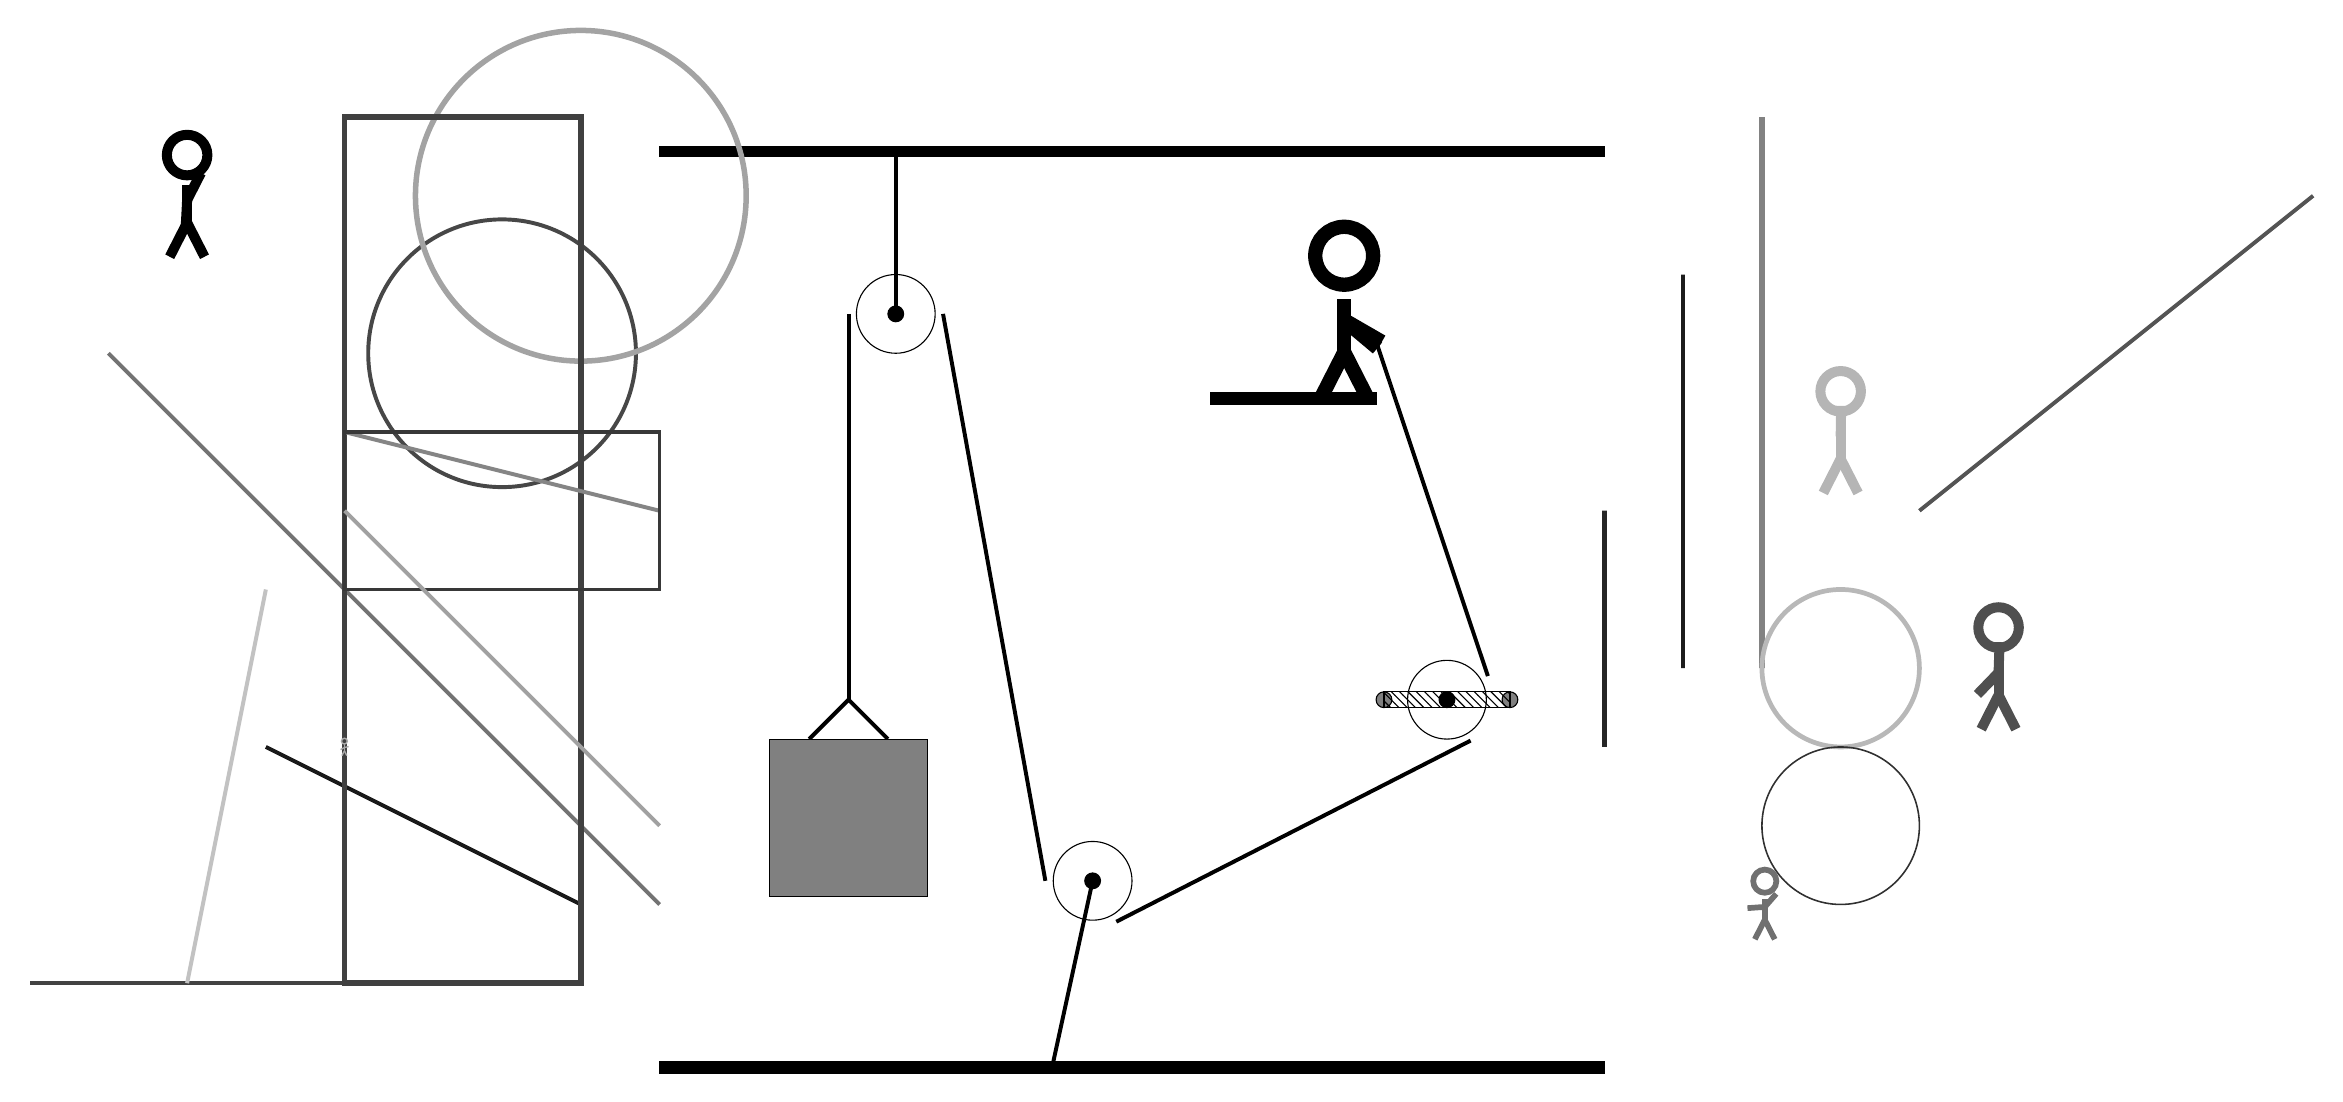
\begin{tikzpicture}
			%%%%% START %%%%%
			
			\draw[fill=black] (-2, 11.5) rectangle (10, 11.625);
			
			\draw (1, 9.5) circle (0.5);
			\draw[fill=black] (1, 9.5) circle (0.1);
			\draw[line width=0.5mm] (1, 11.5) -- (1, 9.5);
			
			\draw (3.5, 2.3) circle (0.5);
			\draw[fill=black] (3.5, 2.3) circle (0.1);
			\draw[line width=0.5mm] (3.5, 2.3) -- (3.0, 0);
			
			\draw[fill=white](8, 4.6) circle (0.5);
			\draw[fill=black] (8, 4.6) circle (0.1);
			\draw[fill=black!50] (8.8, 4.6) circle (0.1);
			\draw[fill=black!50] (7.2, 4.6) circle (0.1);
			\draw[pattern=north west lines, pattern color=black] (7.2, 4.7) rectangle (8.8, 4.5);
			
			\node[line width=0.7mm, color=black!29] at (13, 8) {\Strichmaxerl[7][90][89]};
			
			\draw[line width=0.5mm, color=black!74](-4, 1) -- (-10, 1);
			\draw [line width=0.5mm, color=black!72](-4, 9) circle (1.7);
			\draw[line width=0.5mm, color=black!24](-7, 6) -- (-8, 1);
			
			\draw[line width=0.5mm, color=black!67](14, 7) -- (19, 11);
			
			\node[line width=0.5mm, color=black!100] at (-8, 11) {\Strichmaxerl[7][87][63]};
			
			\draw[line width=0.5mm, color=black!90](-7, 4) -- (-3, 2);
			
			\draw[line width=0.5mm, color=black!55](-2, 2) -- (-9, 9);
			\node[line width=0.3mm, color=black!69] at (15, 5) {\Strichmaxerl[7][46][88]};
			\draw [line width=0.7mm, color=black!36](-3, 11) circle (2.1);
			
			\draw[line width=0.7mm, color=black!85] (10, 4) rectangle (10, 7);
			
			\draw[line width=0.7mm, color=black!75] (-3, 12) rectangle (-6, 1);
			\draw[line width=0.5mm, color=black!48](-2, 7) -- (-6, 8);
			
			\draw[line width=0.4mm, color=black!78] (-2, 6) rectangle (-6, 8);
			\node[line width=0.2mm, color=black!33] at (-6, 4) {\Strichmaxerl[1][28][14]};
			\draw[line width=0.7mm, color=black!49] (12, 5) rectangle (12, 12);
			
			\draw [line width=0.6mm, color=black!28](13, 5) circle (1.0);
			\draw[line width=0.5mm, color=black!89] (11, 10) rectangle (11, 5);
			\draw [line width=0.2mm, color=black!81](13, 3) circle (1.0);
			
			\node[line width=0.3mm, color=black!56] at (12, 2) {\Strichmaxerl[4][4][49]};
			\draw[line width=0.5mm, color=black!42](-7, 7) -- (-7, 7);
			
			\draw[line width=0.5mm, color=black!37](-2, 3) -- (-6, 7);
			
			\draw[line width=0.5mm](-0.1, 4.1) --  (0.4, 4.6) -- (0.9, 4.1);
			\draw[fill=black!50] (-0.6, 4.1) rectangle (1.4, 2.1);
			
			\draw[line width=0.5mm](0.4, 9.5) -- (0.4, 4.6);
			\centerarc[line width=0.5mm](1, 9.5)(180:0:0.6)
			\draw[line width=0.5mm](1.6, 9.5) -- (2.9, 2.3);
			\centerarc[line width=0.5mm](3.5, 2.3)(180:300:0.6);
			\draw[line width=0.5mm](3.8, 1.7804) -- (8.3, 4.0804);
			\centerarc[line width=0.5mm](8, 4.6)(300:390:0.6);
			\draw[line width=0.5mm](8.5196, 4.9) -- (7.05, 9.3);
			
			\node at (6.75, 9.5) {\Strichmaxerl[10][-220][-30]};
			\draw[fill=black] (5, 8.5) rectangle (7.1, 8.35);
			
			\draw[fill=black] (-2, 0) rectangle (10, -0.15);
			
			%%%%% END %%%%%
		\end{tikzpicture}
	\end{figure}	
\end{document}